\documentclass[journal]{IEEEtran}
\usepackage{amsmath}
\usepackage{gensymb}
\usepackage{graphicx} % Required for inserting images
\usepackage{tabularx}
\usepackage{listings} 
\usepackage{ltablex}
\usepackage{upgreek}
\usepackage{multirow}
\usepackage{hyperref}
\usepackage{float}

\begin{document}

\begin{center}
	\Large Garden Automated Rain/Daylight Executed by Near-Infrared Sensing \break

	\large Nicholas Chitty, Brendan College, Scott Peirce, Justin Pham-Trinh \break

	\large University of Central Florida, Dept. of Electrical and Computer Engineering, Orlando,
	Florida, 32816-2450
\end{center}

\begin{abstract}
   Advances in both electronics and optoelectronics have greatly increased the accessibility
of complex devices. This paper will demonstrate the feasibility of installing a near infrared
scanning spectrometer into any yard, garden, or greenhouse for soil characterization with no need
for infrastructure to support it, except a water hose. Self-sufficiency will be achieved through solar
energy collection and battery storage. System control will be achieved via an electronic microcontroller.
The soil characteristics measured will be Moisture Content, Phosphorous, and Carbon. This data may be
interpreted by the microcontroller to adjust the garden bed which the device is installed on and make
the data accessible to the user. 
\end{abstract}

\section{Introduction}
\IEEEPARstart{S}{o}il characterization is shifting away from laboratory analysis and toward optical
sensing. While chemistry experiments may determine soil composition with high degrees of accuracy,
they are unfeasible on economies of scale. Every sample must be preserved for a trip back to the lab,
and lab work takes time and other valuable resources to evaluate even a single sample. Some lab work
can be done in the field, but this limits the accuracy and types of elements that can be investigated.
Spectral sensing offers two advantages: results returned by devices are limited only by scanning speeds
and computing power, and scanning covers a lot of ground, rather than a small spot. There is now a
market for precision agricultural technology, and research is ongoing to improve the efficiency of
these devices.

Soil Scanners, like those developed by AgroCares, MertControl Group, and NPC Agro, typically employ
a broadband light source to probe the soil, then collect reflectance data using an array of photodetectors.
Relevant spectral data is mostly contained within the near and mid infrared regimes. However, Moisture
Content, Carbon, Phosphorous, and pH all have spectral fingerprints that can be detected within the visible
and near infrared spectrum. A reflectance scanning spectrometer with a broadband source and one or two
cheap detectors covering the 400-1700nm range are sufficient to measure these variables\cite{Mouazen2007}.

In addition to professional products and services, hobby project forums are also advancing the
accessibility of complex systems. Hydroponic gardeners are experimenting with water distribution systems,
Arduino programmers have created a market for cheap network communication devices, and optoelectronics
hobbyists have even developed DIY optical spectrometers\cite{Cao}. These projects represent a major development in
engineering activity. It is now possible for a small, poorly funded team of amateurs to create a device
with not only mechanical function, but also wireless control and user interfacing. 

\section{Materials and Methods}

This project is intended to integrate system controls, power, and the web, all to provide 
a "set it and forget it" home gardening experience. There are many different communication protocols
such as Bluetooth, Zigbee, Thread, and even short-range/long-range protocol. For this project WiFi is suitable
because of its decreased bandwidth and because not much data is be produced or received.

Another important aspect is data storage and web usage. This is important for maximizing scanning resolution
and presenting analysis to the user. The web system communicates with the microcontroller through transmission control protocol.
Transmission control protocol is a standard to establish and maintain a network connection to 
exchange data. The web system also has a 16GB database to store data and has the ability to support 
multiple garden beds in a scaled solution. As mentioned before, the web system has a feature to 
allow the user to adjust settings but also read the data that is stored. An important factor to any 
environment is the weather, knowing when it might be cold, hot, or even rain outside. The web system 
will communicate using HTTP requests with a weather service to receive updates that will be passed along 
to the user, when needed.

Solar power has been a growing source of energy in recent years and still continues to be with new 
developments and breakthroughs with solar technology. A lot of systems nowadays are solar powered, but 
these products are not constantly in use, they have to turn off eventually. When the product is off the 
solar panel can still collect energy which is stored in a battery for conservation. This project will be 
the same, battery powered but charged through solar panels.

There are several means of achieving near infrared spectrometry. In this case, the best option is to build a reflectance 
scanning spectrometer. While transmission gratings are substantially cheaper, they lose much optical power 
outside of the zero order, which is unusable due to spectral overlap. A reflectance grating allows for 
maximum signal to noise ratio. The next challenge is how to scan. A rotational scanner was considered and 
rejected, on account of the difficulties of mechanical design. A rotating mount would have to have high 
precision movement, be rigid to ensure maintained optical alignment, and would greatly increase the 
complexity of optical alignment. A linear actuator rail with a stepper motor offers a better solution. 
Rather than change the path of the beam, it changes the position of the photodetectors along the axis of 
diffraction. This allows for rectangular geometries, reducing the mechanical complexity of the optical 
mounts, and in turn, reducing cost.\\

The following are the goals the team set at the outset of the project. Starting with the Primary Goals:
\begin{enumerate}
	\item A spectrometer that operates in the 400nm to 1700nm band with a spectral resolution less
	      than 50nm and signal-to-noise ratio greater than 2.
	\item The ability to automatically feed water into the garden bed.
	\item A microcontroller that serves data to the user.
\end{enumerate}
Moving on, the team had Stretch Goals:
\begin{enumerate}
	\item Power the garden bed completely from solar and battery power.
	\item Serve data to the user via a website.
\end{enumerate}

\section{High-Level Design}

Based on the goals listed above this section will discuss the high-level thought
process the team undertook in achieving those goals.
\begin{figure}[H]
	\centering
	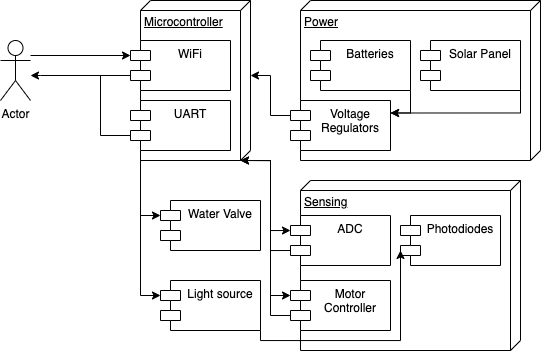
\includegraphics[width=\linewidth]{images/Flowchart.png}
	\label{fig:flowchart}
	\caption{The large systems and their interfaces and submodules}
\end{figure}
In the diagram above, the actor is any user. The team labelled both UART and WiFi blocks as interfaces to the user
because as of the time of writing, the web server is not serving live data. In the figure, the sensing block represents the spectrometer.
\subsection{Controller Subsystem}
The controller subsystem handles all of the I/O between each subsystem, control other ICs, records and stores sensing data, as well as commands and controls the overall system. It performs these actions while only sipping power from the battery, and has wireless capability. A real-time operating system (RTOS) was needed to schedule and supervise the tasks needed to operate a spectrometer, tend to the user's flora, and communicate with the user and APIs wirelessly. All of this was relatively low-cost, this owed to the fact that no data processing takes place on-board the controller subsystem. The controller commands the sensing subsystem to send it data, and simply stores this data to be interpreted at a later time.

\begin{figure}[H]
   \centering
   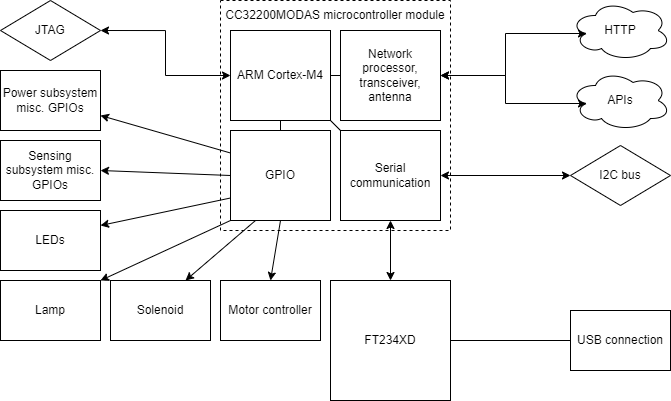
\includegraphics[width=\linewidth]{images/control-block-diagram.png}
   \label{fig:control-block-diagram}
   \caption{Controller subsystem block diagram.}
\end{figure}

% Why the MCU connects to the internet
In order for the system to be as self and power efficient as possible from an end-user perspective, the 
team decided to use a low-power, Internet-of-Things (IoT)-focused wireless microcontroller. To make the 
process of operating the product as hands-off as possible to end-users, the microcontroller operates 
in Access Point (AP) mode to serve information to the user's mobile device. Our product does not produce 
or receive large amounts of data, or need complicated control schema for the various subsystems---and with 
power budget being a major concern, the team chose a product that would fit the bill.
\subsection{Spectrometer} 
The spectrometer employs a small tungsten bulb to cover the spectral range of interest. Light from the bulb 
is directed onto the soil and scattered into a fiber collimator. The collimating head couples the light into 
a fiber patch cable, which guides the light into the dark spectrometer housing. There it is reflected off a 
diffraction grating and focused onto two photodiodes. One Si photodiode covers the visible range, one InGaAs 
covers the near infrared range. These are held in position by a linear rail actuator. The current from the 
diodes is amplified and converted to voltage so that it can be detected, then the microcontroller records the 
amplitude of the signal and the position of the photodiode. The spectral data is then applied to the board logic 
for control, as well as sent to the user for display. See below for a diagram showing the path of information 
through the system.
\begin{figure}[H]
    \centering
    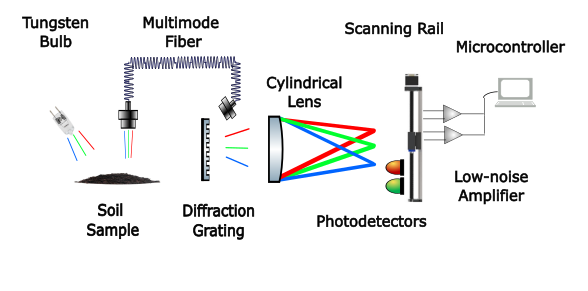
\includegraphics[scale=0.5]{images/Schematic Diagram 2.png}
    \label{fig:sensing-block}
    \caption{Diagram showing the major components of the sensing subsystem.}
\end{figure}
\section{Major Components} \label{sec:major-components}
% How the MCU connects to the internet (local network, LAN -> NAT -> WAN, TCP stack)
\subsection{Microcontroller}
The Texas Instruments CC3220-series (hence referred to as the "CC3220", the "MCU", or the "microcontroller") of microcontrollers are WiFi-enabled chips with an ARM Cortex-M4 central processor and a WiFi network processor, along with many useful peripherals and power management modules. This series of processors is delivered alongside a software development kit (SDK) provided by Texas Instruments to ease the development of IoT applications. The CC3220 is capable of running on bare metal, or with a Real-time Operating System (RTOS), allowing organization and scheduling of various tasks.

The CC3220's WiFi network processor (NWP) supports 802.11b/g/n, SmartConfig provisioning, IPv4 and IPv6. The NWP also has the ability to host an internal HTTP/HTTPS server, and contains its own filesystem.
\subsection{Optics}
When selecting photodetectors, the relevant concerns were sensitivity, effective area, and cost. For a Si photodiode, our team selected the BPX 61 by Newark, since it was the cheapest model and met our needs. The InGaAs diodes available were exceptionally small. Due to our concerns over signal to noise ratio, we opted for a model with a large effective area, the Thorlabs 0800-3111-011.

Tungsten bulbs emit a broad spectrum, far into the infrared. They also come in small package sizes that emit a lot of light for reasonable power consumption. Our bulb, the Osram 54262 runs at 20 Watts of electrical power. This is supplied directly from the battery, though controlled by the microcontroller. The result is 350 lumens, mostly directed onto the soil.

The team needed a linear rail with a carriage mount that the sensors could be mounted to. We selected a 50mm long rail with a screw-turned mount run by a NEMA11 stepper motor.
\subsection{Water valve}
As part of the goals, the team wanted to be able to control the flow of water into the plant bed. To accomplish this, a solenoid valve was chosen whose rated pressure was well specificied for use with home water pressures.
\section{Hardware Design}
In \autoref{sec:major-components}, a high level overview of components and features were given. This section will discuss the implementation details of the chosen components.
\subsection{Spectrometer}
Five components from the spectrometer required design: the light collection system, the diffraction grating, the cylindrical lens, the actuator rail, and the analog-to-digital converter. The system was complemented with other components, such as the housing and photodiodes, however their requirements were less strict and could be satisfied with minimal design beforehand. 
\subsubsection{Light Collection}
The light source is connected via a Darlington transistor and driven with a 12V supply at \~{}1.7A. As this is too much electrical power for the digital controls on the board, the Darlington transistor will isolate this electrical supply. The light from the bulb shines on a patch of soil and reflects onto the fiber head collimator. In order to maximize the effect of reflectance on the sample, the bulb is seated in a reflective metal tube which shields reflections from entering the fiber head.
\begin{figure}[H]
    \centering
    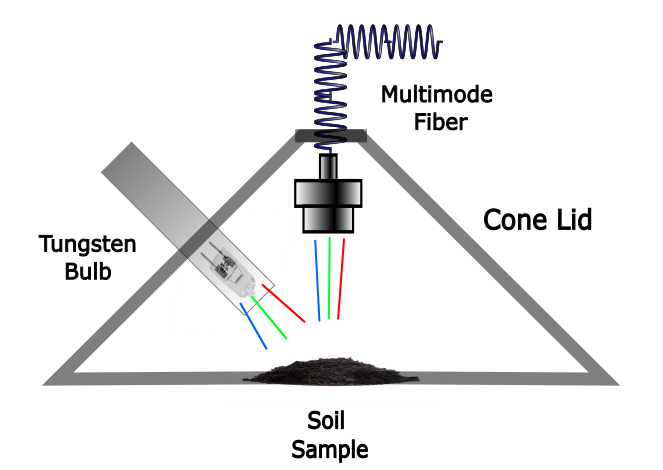
\includegraphics[scale=0.4]{images/Light Collection.png}
    \label{fig:Light-Collection-Diagram}
    \caption{Conical frame for reflecting the light off the soil}
\end{figure}
\subsubsection{Diffraction Grating}
Reflective diffraction gratings disperse light at an angle proportional to wavelength according to the classic grating equation,
\begin{equation}
    m\lambda = d(sin\alpha + sin\beta)
\end{equation}
where m stands for diffraction order, $\lambda$ refers to wavelength, d refers to grating spacing in grooves/mm, and $\alpha$ and $\beta$ stand for input and output angles respectively. Below, the first three orders of diffraction are solved for a beam with wavelengths from 400nm to 1700nm on a grating with 600 grooves/mm. The model allows testing for beams at different incident angles. 50\textdegree \: from normal was optimal, since it allowed the first order reflection to spread widely without coming back into the incident beam. The dispersion covers 47\textdegree.
\begin{figure}[H]
    \centering
    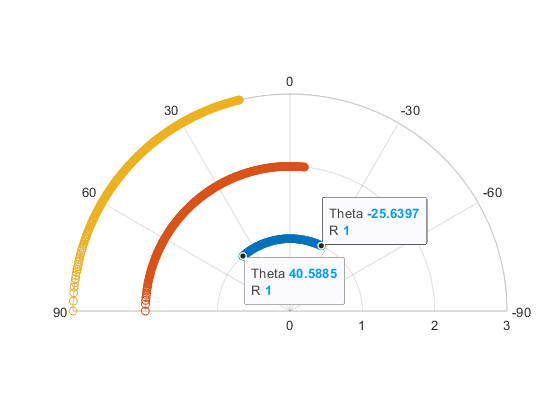
\includegraphics[scale=0.5]{images/PolarPlot.png}
    \label{fig:diffraction-angle}
    \caption{The diffraction angle of 1st through 3rd order diffractions. Note: higher orders have reduced power, negating the effect of overlap}
\end{figure}
\subsubsection{Cylindrical Lens}
Light entering the spectrometer housing exits the fiber patch cable through a collimator with matching numerical aperture. This expands the beam to a diameter of 1.7mm, shining a circular image away towards the diode rail. Ideally, the light would be focused to a point at the photodetector, where the optical power of a single wavelength would be measured. Without optics, a large circle with \~{}1.7mm diameter reaches the rail. To fix this, a lens is positioned just far enough in front of the grating for the incident beam to clear its edge at 50\textdegree from normal to the grating. The lens is cylindrical, focusing the light along the horizontal axis but not along the vertical axis. With the rail positioned right at the focal length of 50mm, the beam focuses neatly along the rail.
\begin{figure}[H]
    \centering
    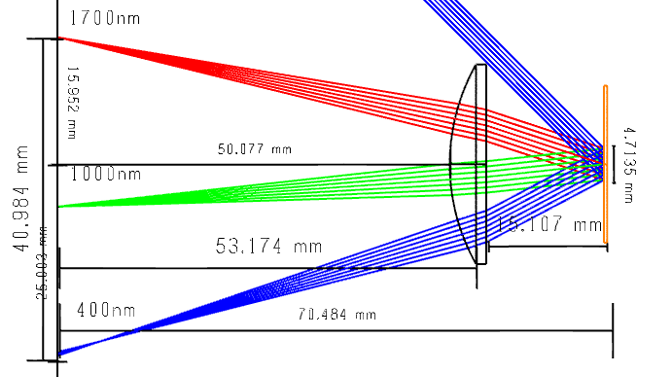
\includegraphics[width=\linewidth]{images/RayTrace.png}
    \label{fig:housing-ray-trace}
    \caption{Ray trace of the idealized beam path through the housing}
\end{figure}
The spot size of an idealized raytrace yields 27 $\mu $m, with \~{}30$\mu $m between spot centers. This is excellent, since the airy disk suggested by the ray trace is within an order of magnitude. This means the arrangement of the components will not raise the lower limit of the spectral resolution above 2nm, although it is doubtful the nonideal system will achieve such precision. 
\begin{figure}[H]
    \centering
    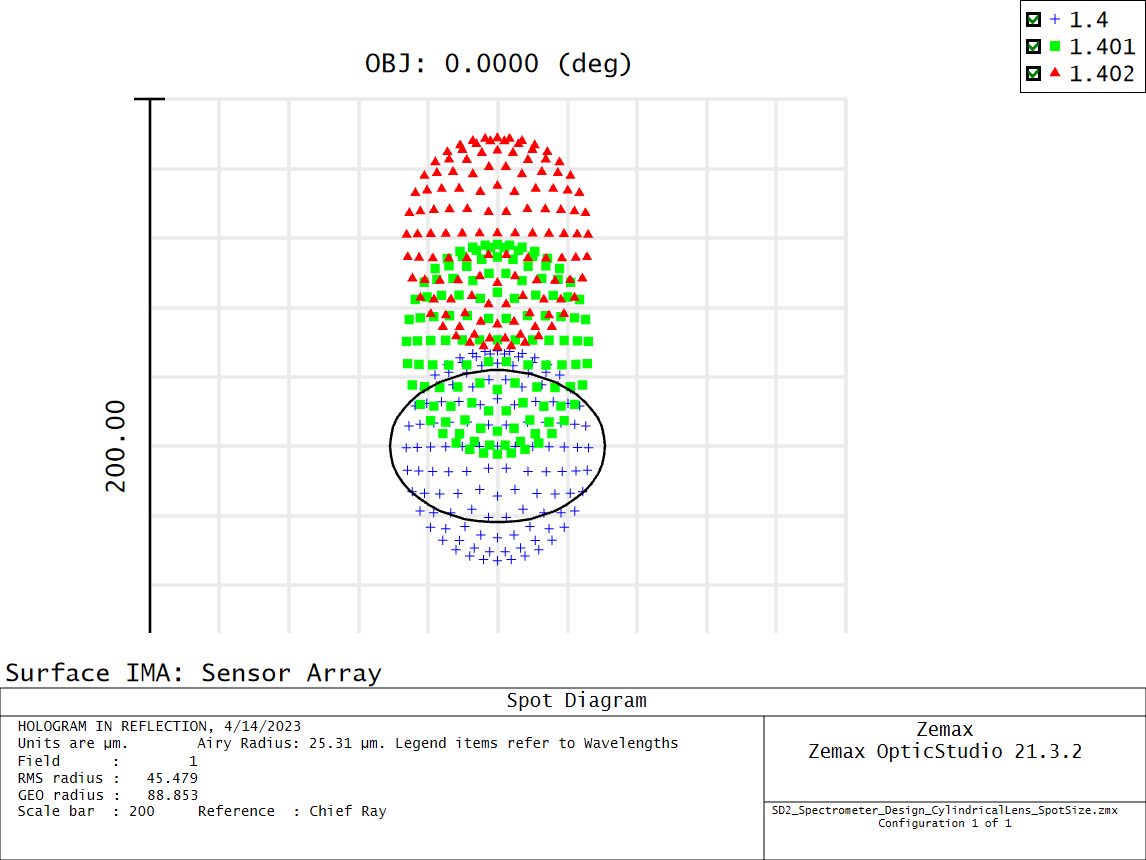
\includegraphics[width=\linewidth]{images/SpotDiagram.png}
    \label{fig:spot-size-diagram}
    \caption{Spot size diagram of three wavelengths focused at the linear rail}
\end{figure}
\subsubsection{Linear Rail Actuator}
Given that there is \~{}30$\mu $m between the center of each focused wavelength spot, and wavelengths range from 400nm to 1700nm the minimum stroke length needed for the linear rail is:
\begin{equation}
    30\mu m*(1700-400) = 39 mm
\end{equation}
Which agrees with the ray trace in Figure 6, there labeled 40.984mm.

The rail has a stepper motor which engages rotation of a central rotor using four electromagnets to adjust the position of the rotor gear teeth by one quarter the width of a tooth. The Rattmmotor linear rail in this system uses the NEMA11, which has a minimum step angle of 1.8\textdegree. The rotor shaft has a mount that is moved up and down along the shaft threading. The pitch angle of this threading is such that for every full rotation, the mount moves 1mm. Therefore, the minimum step size is
\begin{equation}
    d = (\text{Thread pitch})*(\text{Pulse count})*(\frac{\text{Step angle}}{360\text{\textdegree}})
\end{equation}
\begin{equation}
    d = 1 mm*(1)(\frac{1.8}{360}) = 5\mu m
\end{equation}
\subsubsection{Analog to Digital Conversion}
The optical power passing into the housing is above 500$\mu $W when the bulb is fully exposed to the fiber input head. At 50mm from the fiber head, with \~{}50\textdegree \: of dispersion, that drops to just above 10$\mu $W. By removing the fiber input head from in front of the bulb and scattering light off a soil sample, the power drops below what an optical power meter can reliably detect. 

It is at this point that the spectrometer design enters the electrical domain. Due to the photosensitive device being a photodiode where the current is a result of the optical power on the sensitive area, the team built a current-to-voltage converter which would be fed into the analog-to-digital converter. The primary issue at this point is just how small the optical power of the light is. Given that the sensors have a translation of 1nA/1mW of power, a design for a high gain, low noise converter was needed. 100e6 gain was chosen, meaning that 1nA would translate to 100mV, which is over double the resolution of our 16-bit ADC.

\begin{figure}[H]
    \centering
    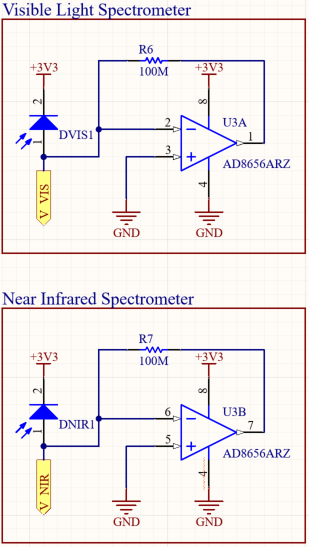
\includegraphics[height=.25\textheight]{images/SensorSchematics.PNG}
    \label{fig:sensor-schematic}
    \caption{The schematics for the current-to-voltage converter.}
\end{figure}
The net labelled \verb|V_NIR| and \verb|V_VIS| are sandwiched between ground planes on their track
to the ADC to reduce noise caused by electrostatic discharge or other analog signals (such as the
motor current). Before being read by the ADC the team designed a low pass filter to try to attenuate
the noise above 60Hz. The value of 60Hz was chosen as the cut off frequency because during
testing the oscilloscope showed a signal frequency in that range that would be detrimental to the
readings.

The sensing subsystem contains a Texas Instruments ADS 7142 ADC. The ADS 7142 is an IoT-focused nanowatt ADC with 2 external channels, an I2C interface, a sampling frequency of 140ksps, and an effective resolution of 16 bits in High-precision Mode. This ADC is able to measure between 0 and 3.3 V from the output of the sensing subsystem's photodiode op-amp circuit.

% How the MCU gets data from sensors (ADC, cont.)
Each photodiode's circuit produces a voltage between 0 and 3.3 V. The 16-bit ADC provides for an input of the same range, therefore, the resolution of the ADC is calculated below:
\begin{equation}
	\frac{(3.3 - 0)\,\mathrm{V}}{2^{16}\,\mathrm{steps}} =
	50.35\,\mathrm{\mu V}/\mathrm{step}
\end{equation}
These steps are used to measure OH composition and nutrients in the soil. The MCU directly controls GPIO and bit-bang values to the stepper motor controlling the position of the photodiodes allowing them to measure the full range of spectral values.
\subsection{Printed Circuit Board} The controller subsystem was developed and implemented on a Texas Instruments LaunchPad development board. An initial control printed circuit board (PCB) was designed, fabricated, and assembled (partially seen in \ref{fig:mcu_v1_cpwg}). The chip version of the CC3220 (CC3220S) was used requiring a 4-layer impedance-controller PCB, with waveguide and external antenna, as well as oscillators, numerous bypass capacitors, and inductors.

\begin{figure}[H]
   \centering
   \label{fig:mcu_v1_cpwg}
   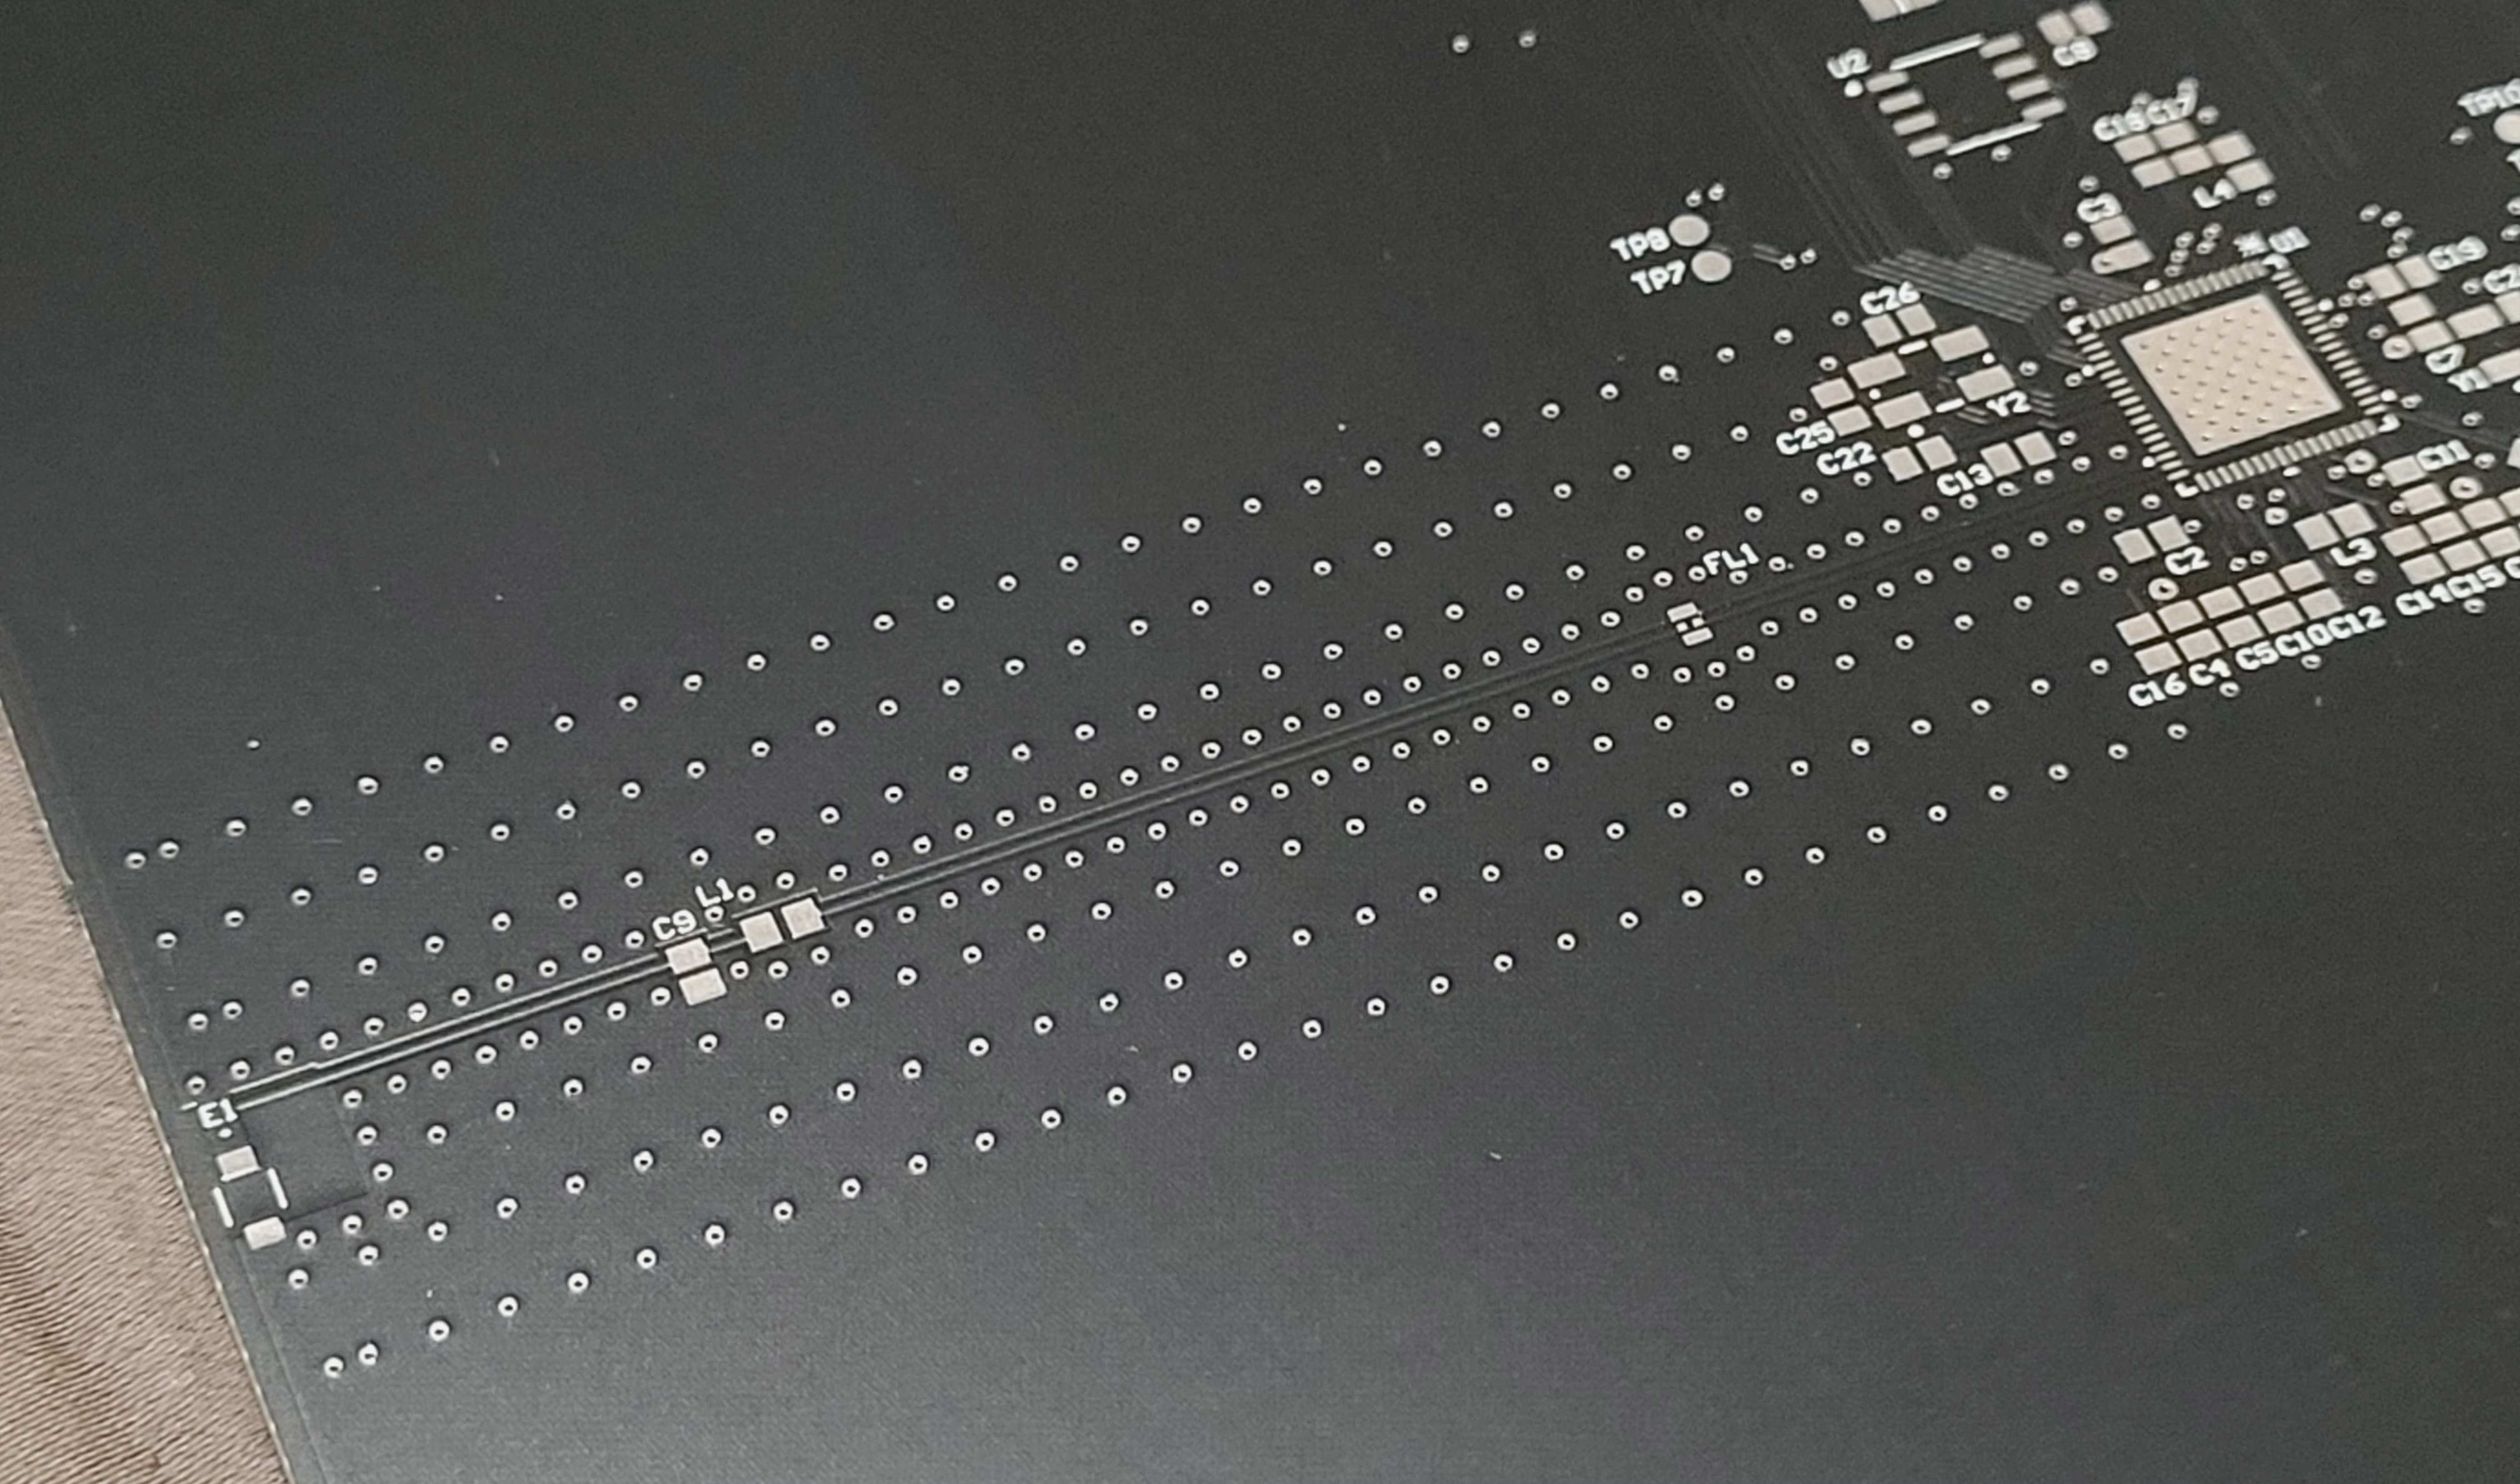
\includegraphics[width=\linewidth]{images/mcu_v1_cpwg.jpg}
   \caption{The coplanar waveguide designed to carry a 2.4 GHz signal surrounded by via fencing.}
\end{figure}

A revised PCB (seen in \ref{fig:mcu_pcb_v2}) was designed using the module version of the CC3220 (CC3220MODAS). The PCB design was simplified, requiring only a few bypass capacitors instead of the numerous other components to support the microcontroller found on the first revision of the board. All other components found on the first version of the board were kept (e.g. molex connectors, LEDs, JTAG connector, FT234XD, etc.). In addition, pinouts were added for GPIO, I2C, and power to aid in debugging.

\begin{figure}[H]
   \centering
   \label{fig:mcu_pcb_v2}
   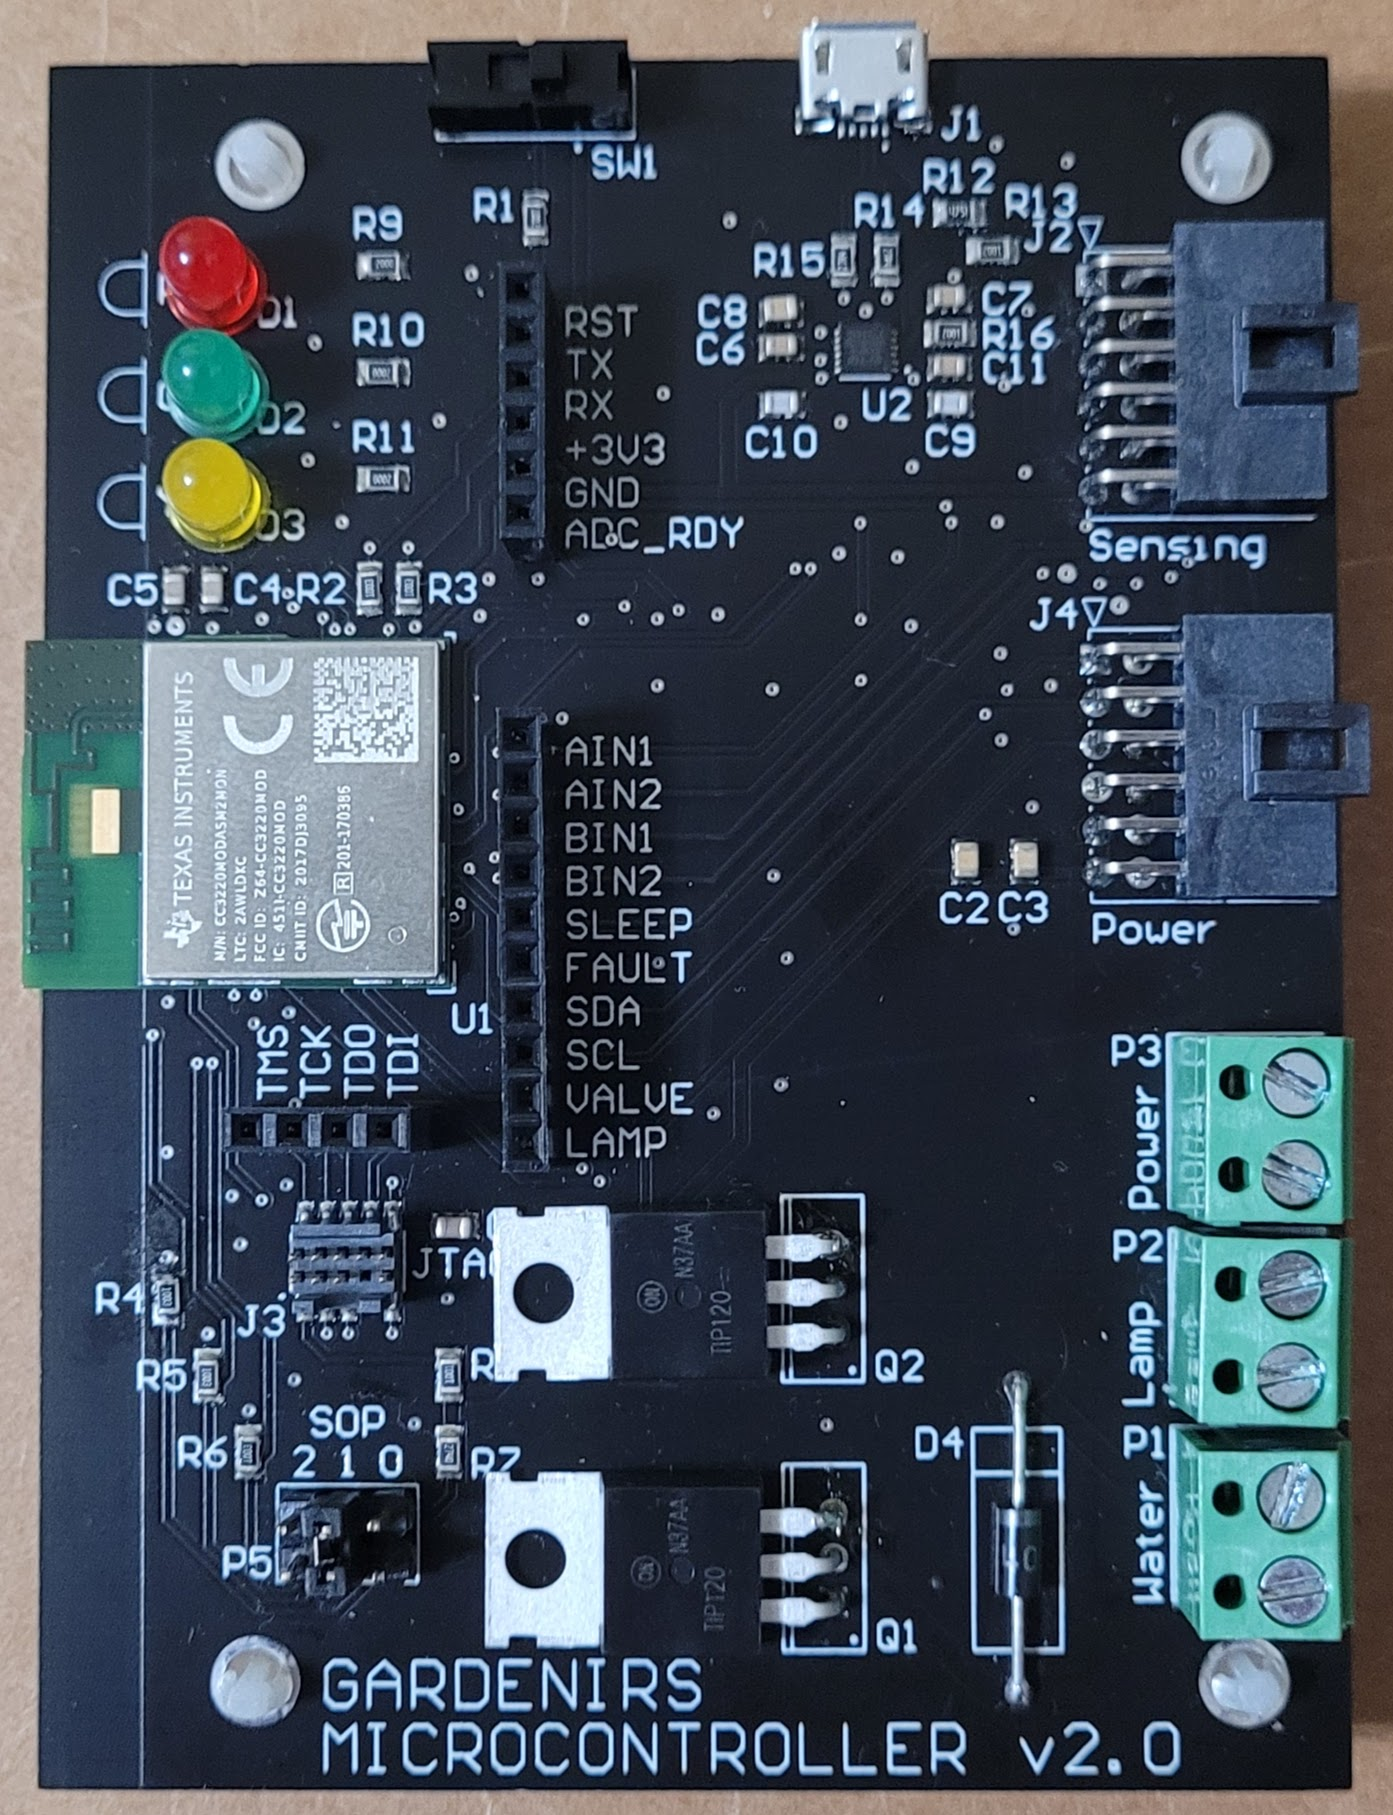
\includegraphics[width=\linewidth]{images/mcu_pcb_v2.jpg}
   \caption{Version 2 of the MCU PCB.}
\end{figure}
\subsection{Power Subsystem} \label{sec:power-subsystem}
The components that make up this subsystem in all are the battery, solar panels, voltage regulators, 
and the charge controller. These components together also make our system operate working with other 
subsystems but also helping the other subsystems work together as well. 

\subsection{Battery} \label{sec:battery}
Solely, to make any product or system to operate, power is needed in some type of form. DC power 
connectors, batteries, connection to a direct source, there are many different ways to obtain power 
in order for something to operate. DC power connectors have always been around and have been used 
in many different scenarios for different situations. They give access to constant power easily 
because we are able to simply plug it into a wall outlet and they are also inexpensive. Batteries, 
like the power connectors, also come in differnt forms. Batteries can be made of different materials, 
they can have different ratings, and other features as well. On the other hand, batteries can discharge 
and run out of power. 

In recent years, there has been a rise in energy storage, small and large scale. In 2021 alone, there 
was a 60\% increase in energy storage capacity. This is because of the increase in sustainable energy 
programs, such as solar, that there is a demand in either new or more energy storage, mainly batteries. 
Batteries are being deployed for economic and safety reasons. Battery technology is advancing to become 
more powerful, last longer, and become safer for consumers. In our project, we wanted to incorporate 
energy storage as a way to make our system operate independently. There were many batteries to choose 
from with new battery chemistries rising as well as existing chemistries advancing, but for our system 
we decided to go with a LiFePo4 battery. This was our choice because many reasons including a longer 
life span, they do not require too much maintenance, extremely safe, improved discharge and charge 
efficiency, and so much more. 
\subsection{Solar Panel} \label{sec:solar pane}
Solar technology in general has seen its advances in recent years and increase in demand for solar panels. 
Part of making our system operate independently we went with solar engergy, even though our system is 
battery powered, solar energy is charging the battery. With solar panels, there three different types of 
solar panels, monocrystalline, polycrystalline, and thin-film, all of which differ in material and 
composition, vary in effiencies, and few other aspects. To get the highest efficiency, the solar panels 
that were picked were the monocrystalline.
\subsection{Charge Controller} \label{sec:charge controller}
Working with the battery and the solar panel is the solar charge controller. Simply put, the main role of 
charge controller is to ensure that the battery is not being overcharged. The way solar panels and batteries 
work together is that as the battery is not operating after usage, the solar panels collect energy that 
is brought to the battery to charge. Now if the battery is at full capacity, it is dangerous to continue 
to bring more energy into it because it could damage it and decrease its life span. There are two different 
charge controllers, both of which manage the amount of charge that is going into the battery, maximum power 
point tracking and pulse width modulation. To ensure the highest efficiency as well, we went with the 
maximum power point tracking charge controller.
\subsection{Voltage Regulators} \label{sec:voltage regulator}
Lastly, the voltage regulators. Voltage regulators are and important part to any electronic product because 
similar to the charge controller they manage voltage. The main role of the voltage regulator is the regulate 
voltage, either increasing or decreasing voltage to a specified level that is needed. This is important 
because in houses the standard wall outlet is 12V, but a certain product needs only 5V. Plugging this product 
into the wall directly the product will overcharge and break. Similarly, there are many different types of 
voltage regulators too, all of which operate differently and have different features. In integration, the 
voltage regulators work with all the other subsystems because the components in their system operate on 
differnt voltages. So, from the our 12V battery, it travels to our power PCB and then from there power is 
distrubuted among the rest of the system and sending the appropriate voltages to each component. For this 
project, we decided on a few differnt voltage regulators because some of our other components varied in 
voltages from 3.3V, 5V and 12V. 

\section{Software Detail}
The microntroller serves as the glue holding this design together. In this section the means of
integrating the various subsystems via software will be discussed.
\subsection{Development Model}
An Agile development model was used to program the control subsystem and its various modules. Code reviews were performed on an as-needed basis by a convening of members of the MCU subsystem and the web subsystem teams. Texas Instruments Code Composer Studio v12 was used to program, compile (via TI ARM compiler v20), and debug the C++-based project. GitHub was used as a repository for the project, using GNU Git for version control.

The Meyers' Singleton design pattern was used for most of the classes found in the project repository 
(e.g. for our water solenoid class as seen in \ref{fig:singleton_implementation}). Because the team is 
using a RTOS with a scheduler and threads, it is advantageous to divide and schedule tasks for the different 
submodules of our project. However, one problem the team took into consideration is that there is only one 
physical instance of each submodule. The normal Singleton pattern traditionally has been used when one wants 
only one instance of a class initialized at any one point, but they are not thread-safe. One variation of this 
pattern is the Meyers' Singleton, which guarantees that only one instance of a type is available at any time. 
Initialization of this pattern is thread-safe, and locks can be used to ensure thread safety when accessing 
members of the class. This is accomplished by using a static local variable inside a static member function 
to hold a single instance of the class. The Meyers' Singleton takes advantage of the fact that the initialization 
of static local variables inside functions is guaranteed to be thread-safe. The Meyers' Singleton disallows 
copying and moving of the class, and makes member constructors and destructors private\cite{Meyers}.

% Code style
\lstdefinestyle{mystyle}{
	basicstyle=\ttfamily\footnotesize,
	breakatwhitespace=false,
	breaklines=true,
	captionpos=b,
	keepspaces=true,
	numbers=left,
	numbersep=-15pt,
	showspaces=false,
	showstringspaces=false,
	showtabs=false,
	tabsize=2
}
\lstset{style=mystyle}

\begin{figure}
	\centering
	\label{fig:singleton_implementation}

	\begin{lstlisting}[language=C++]
    class Water { 
        public:
            static Water& instance();

            // Disallow copying
            Water& operator = (const Water&) = delete;
            Water(const Water&) = delete;

            // Disallow moving
            Water& operator = (Water&&) = delete;
            Water(Water&&) = delete;

            // Class functions
        
        private:
            Water();
            ~Water();

            // Class variables
    };
\end{lstlisting}
	\caption{An example of the Meyers' Singleton pattern implementation within the project.}
\end{figure}
\subsection{Data}
As well as being able to see and configure the network settings of the product, the user will be able to see data relating to the OH-levels and common plant nutrient levels as determined by the spectral analysis of the product. For one measurement, 16 bits of data will need to be stored per position from 130 unique positions, per sensor.
\begin{equation}
	\frac{16\,\mathrm{b}}{8\,\mathrm{b/B}}\times 130\,\mathrm{positions} \times 2\,\mathrm{sensors} = 520\,\mathrm{B}
\end{equation}
With 8 Mb of the 32 Mb (1 MiB of the 4 MiB) shared serial flash dedicated to storing results, this allows 2016 measurements stored.
\begin{equation}
	\frac{1\,\mathrm{MiB}}{520\,\mathrm{B/measurement}} = 2016\,\mathrm{measurements}
\end{equation}
Stretching out measurements to be recorded every 15 minutes, this will allow a user to see individual measurements stretching back exactly three weeks.
\begin{equation}
	2016\,\mathrm{measurements} \times \frac{1\,\mathrm{measurement}}{15\,\mathrm{min}} = 30240\,\mathrm{min}
\end{equation}
As a stretch goal these measurements can be aggregated and analyzed, and allow serving trends and predictions to the user.

\subsection{Software Logic Flow} 
\begin{figure}[H]
    \centering
    \label{fig:logic-flow}
    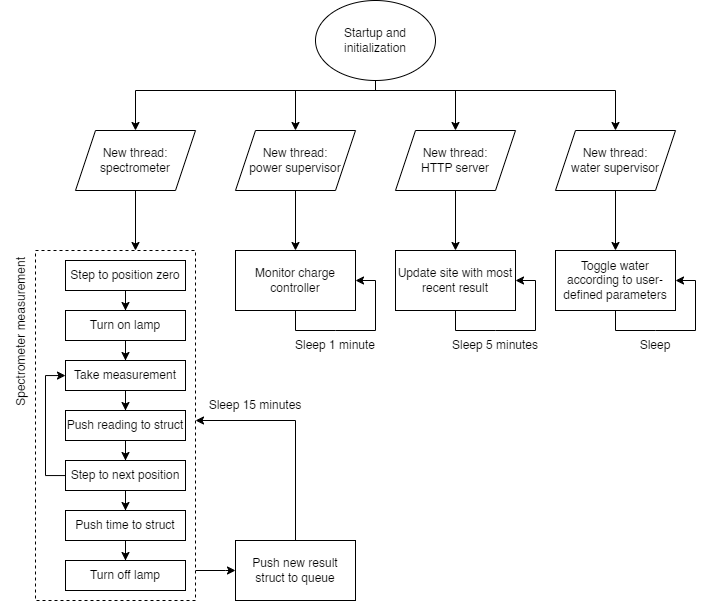
\includegraphics[width=\linewidth]{images/logic-flow.png}
    \caption{Software logic flow diagram}
\end{figure}

The RTOS monitors 4 threads, each dealing with vital functions of the product. 
The first thread deals with the sensing subsytem and operating the spectrometer, 
as well as recording results. When a measurement is needed, the lamp is turned on 
and the spectrometer is stepped through every position to take a voltage reading 
that is placed in a struct. When the last measurement is taken, the light is turned 
off, the time is recorded in the struct, and the measurement struct is pushed to a 
queue. The HTTP server thread reads the results from the queue and posts them for 
the user to see. The power supervisor thread reads from the charge controller every 
minute. If it encouters an unsafe situation, it is able to command the system's power 
state to resolve the situation. Lastly, the water supervisor thread controls the water 
solenoid, turning it on and off according to parameters input by the user.

\subsection{Connection}
The product broadcasts a WLAN in AP mode that allows the user to connect to the product. 
The user is then directed to a web portal hosted by the MCU's internal HTTP server, 
where they will be able to view information, sensing data, and telemetry related to the 
product. Hosting a web interface would allow unanimous adaptation of our product for home users.

\subsection{Libraries}
The C++ standard library (as defined in C++14), the POSIX library, and the Texas 
Instruments SimpleLink CC32xx SDK were used for this project. No 3rd party libraries were used.

% Parameters for connection and how often it tries
\subsection{Weather API Implementation}
As a stretch goal, the user will be able to configure the MCU in Station mode to allow 
it to connect to the user's home WLAN's SSID as a client. The user would still be able 
to access the MCU's web portal and see the same information as they had before. In 
addition, the MCU would be able to access an API to receive weather information and inform 
the user of recommended actions pertaining to their garden bed (e.g. if the system determines 
there will be freezing temperatures overnight, it may suggest to the user to cover the garden bed with a sheet or towel).
\subsection{Motor Controller}
Four GPIO lines are used to control the stepper motor holding the sensing PCB (which includes 
the photodiodes, op-amp circuitry, ADC, motor controller, and connector). Depending on the 
digital values passed to the motor controller, the motor controller is able to control the 
movement direction and speed. The SimpleLink SDK's high-level hardware abstraction layer (HAL) provides 
too long of a delay when changing values in the four GPIO lines. Nanosecond-levels of delay 
were needed, rather than the microsecond levels of delay our team was seeing. Instead of 
using highly-abstracted APIs for control of the motor, the team got as close to hardware as is possible 
with C/C++ and used TI's driverlib driver library specifically for the CC3220. Instead of a simple 
GPIO number being passed to the function, the team had to determine the GPIO port and port-specific 
pin of each input of our motor controller. The driverlib function checks the port for correctness, 
and then performs a system call to write a value directly to memory (in our case, the address of the 
GPIO port). Using driverlib also allows to bit stuffing GPIO pins if they are located on the same 
port---on the second iteration of the board, the motor controller GPIOs were relocated to the same GPIO port 
and bitmasks used to can change all four GPIO pins with one driverlib write function. This allows for toggling a 
single GPIO pin within a period of 350 ns (seen in \ref{fig:gpio_toggle_driverlib}). With a speed of 80 MHz in 
active mode, this would mean we're able to write to GPIO in only 28 processor cycles.
\begin{equation}
	350\,\mathrm{ns} \times (80\times10^6\mathrm{cycles/s}) = 28\,\mathrm{cycles}
\end{equation}
This is a huge accomplishment for our team, especially with a program written in C++ and utilizing HAL.

\begin{figure}[H]
	\centering
	\label{fig:gpio_toggle_driverlib}
	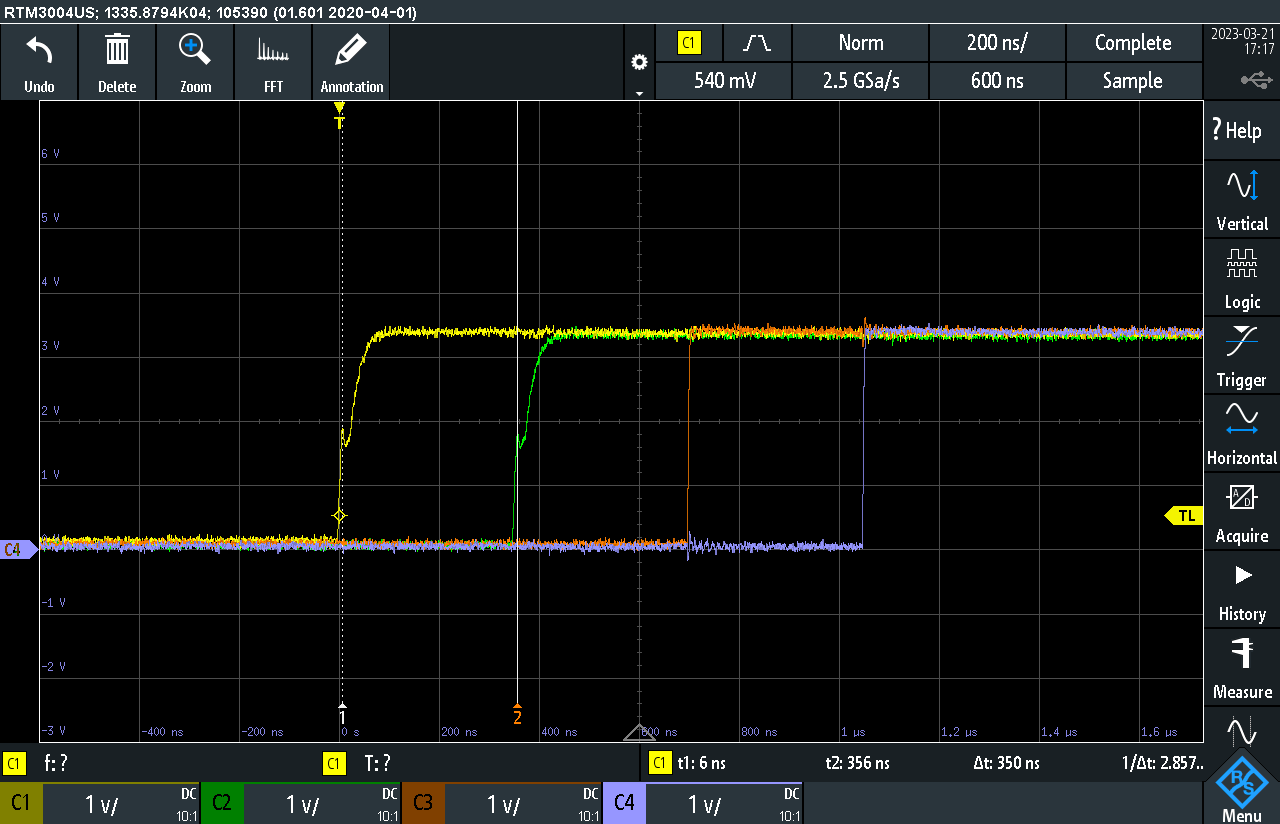
\includegraphics[width=\linewidth]{images/gpio_toggle_driverlib.jpg}
	\caption{Toggling GPIO using driverlib results in a very short (350 ns) delay.}
\end{figure}
To drive a DC motor we similarly needed a device to separate the digital logic from the back emf of the motor. 
This is done through the use of the motor driver. The timing of the signals is the most important part as the 
driver is just using the current and voltage source designed specifically for the motor in the timings given by 
the input pins. Wrong timing leads to the ability to skip tests leading to indeterministic behavior. The issue 
is the the CC32xx SDK abstracts away a lot of the fine tunability of setting hardware registers. To resolve this, 
the team used the specific board's hardware driver implementation to set the output on the pins with a delay of only 28 cycles.
\subsection{Over-the-Air Updates}

\section{Results}
With the garden bed constructed, the power module in working order, and the program loaded onto the microcontroller, 
tests ran smoothly. The spectrometer was first run with a test surface to guarantee its SNR was readable and the 
motor carriage passed along the diffracted beam. With minimal adjustments, the device was ready for scanning. 
Three materials were tested: sandy soil collected outdoors near the university, potting soil and a composted 
manure soil, both purchased from a local hardware store. The scans are presented below.
\begin{figure}[H]
   \centering
   \label{fig:Data1}
   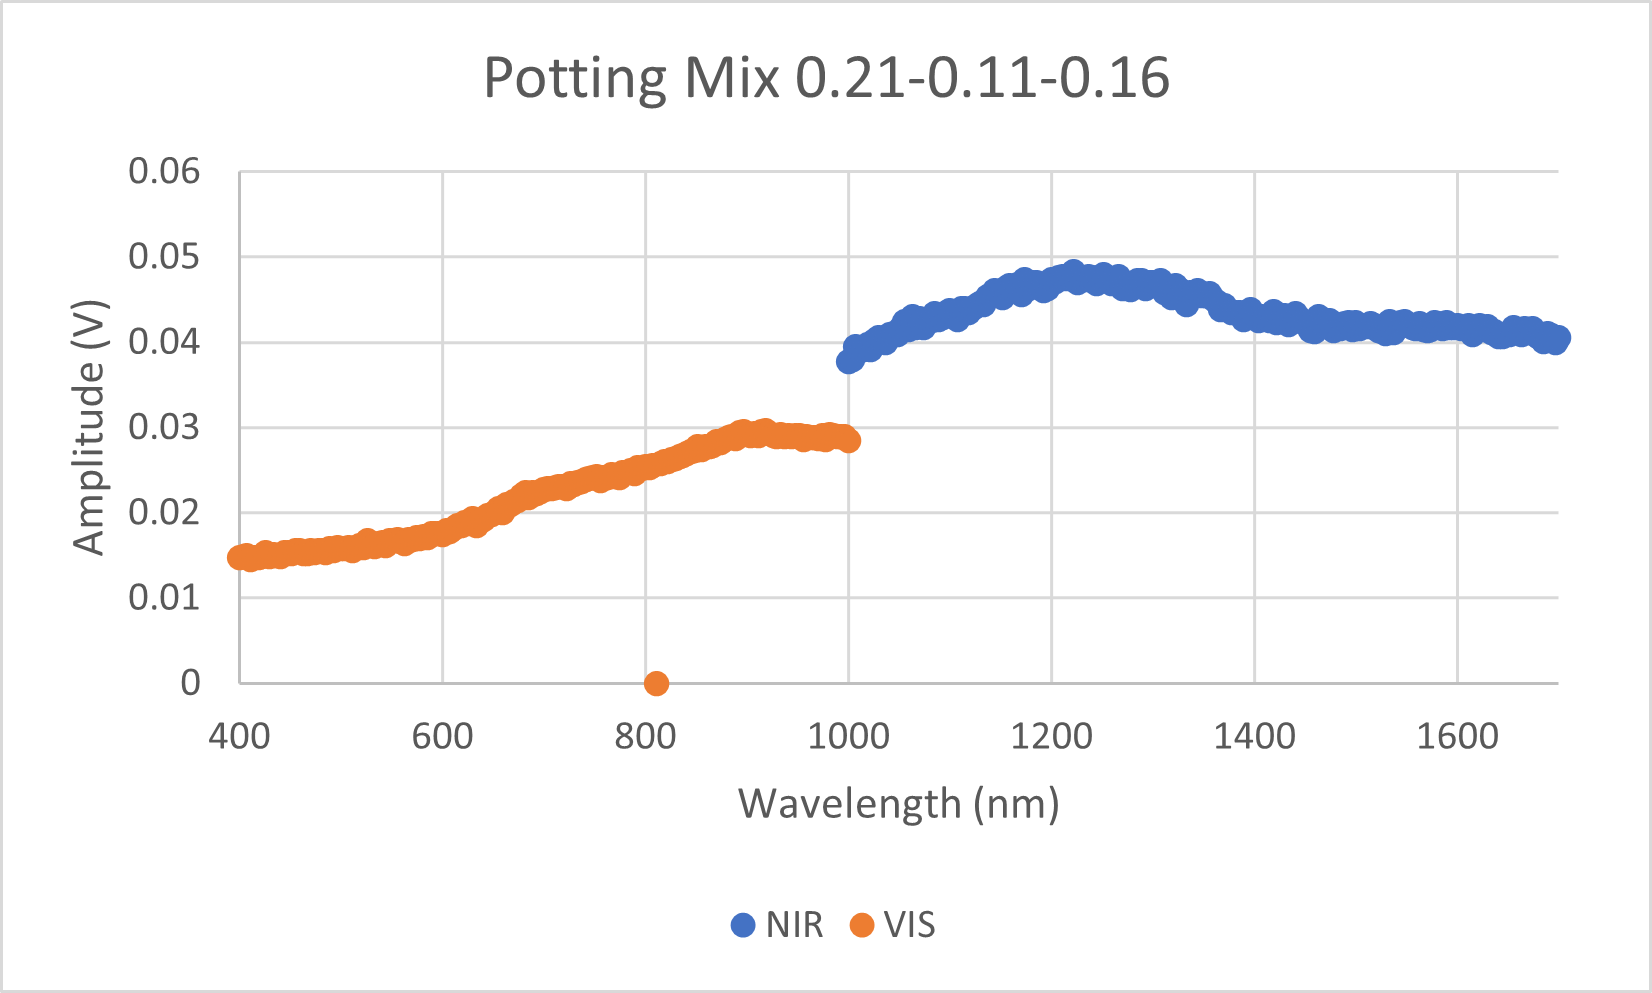
\includegraphics[width=\linewidth]{images/Data1.png}
   \caption{Spectrograph of a fertilized bag of potting mix}
\end{figure}
\begin{figure}[H]
   \centering
   \label{fig:Data2}
   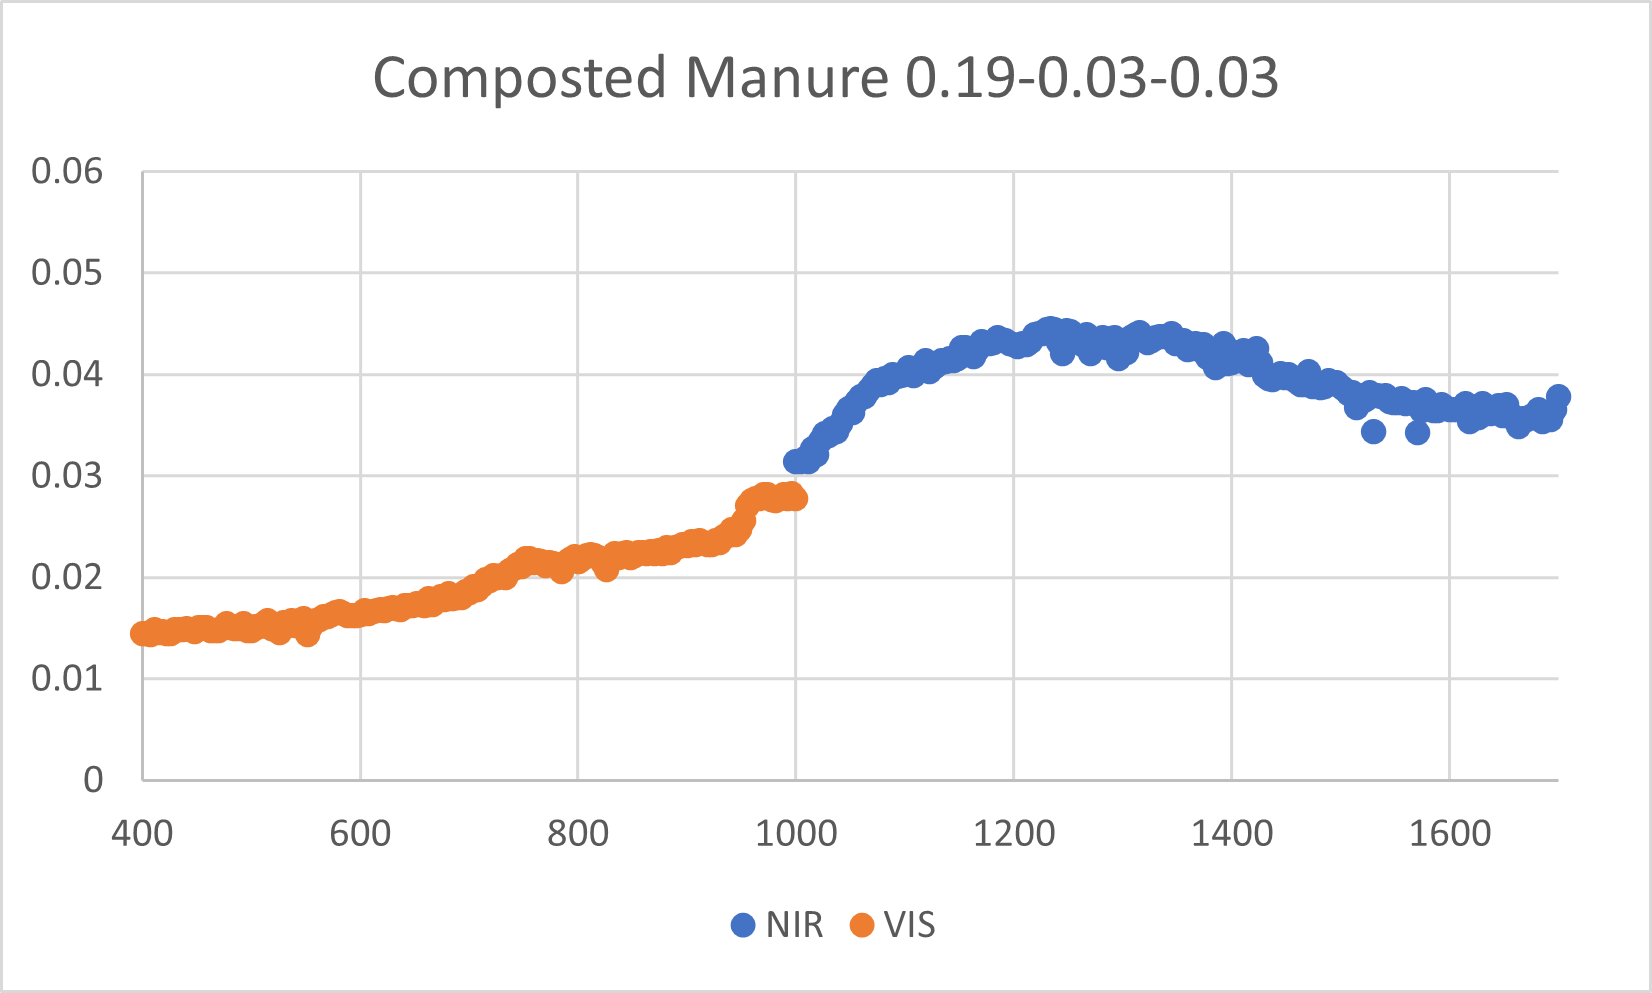
\includegraphics[width=\linewidth]{images/Data2.png}
   \caption{Spectrograph of a bag of compost manure soil}
\end{figure} \begin{figure}[H]
   \centering
   \label{fig:Data3}
   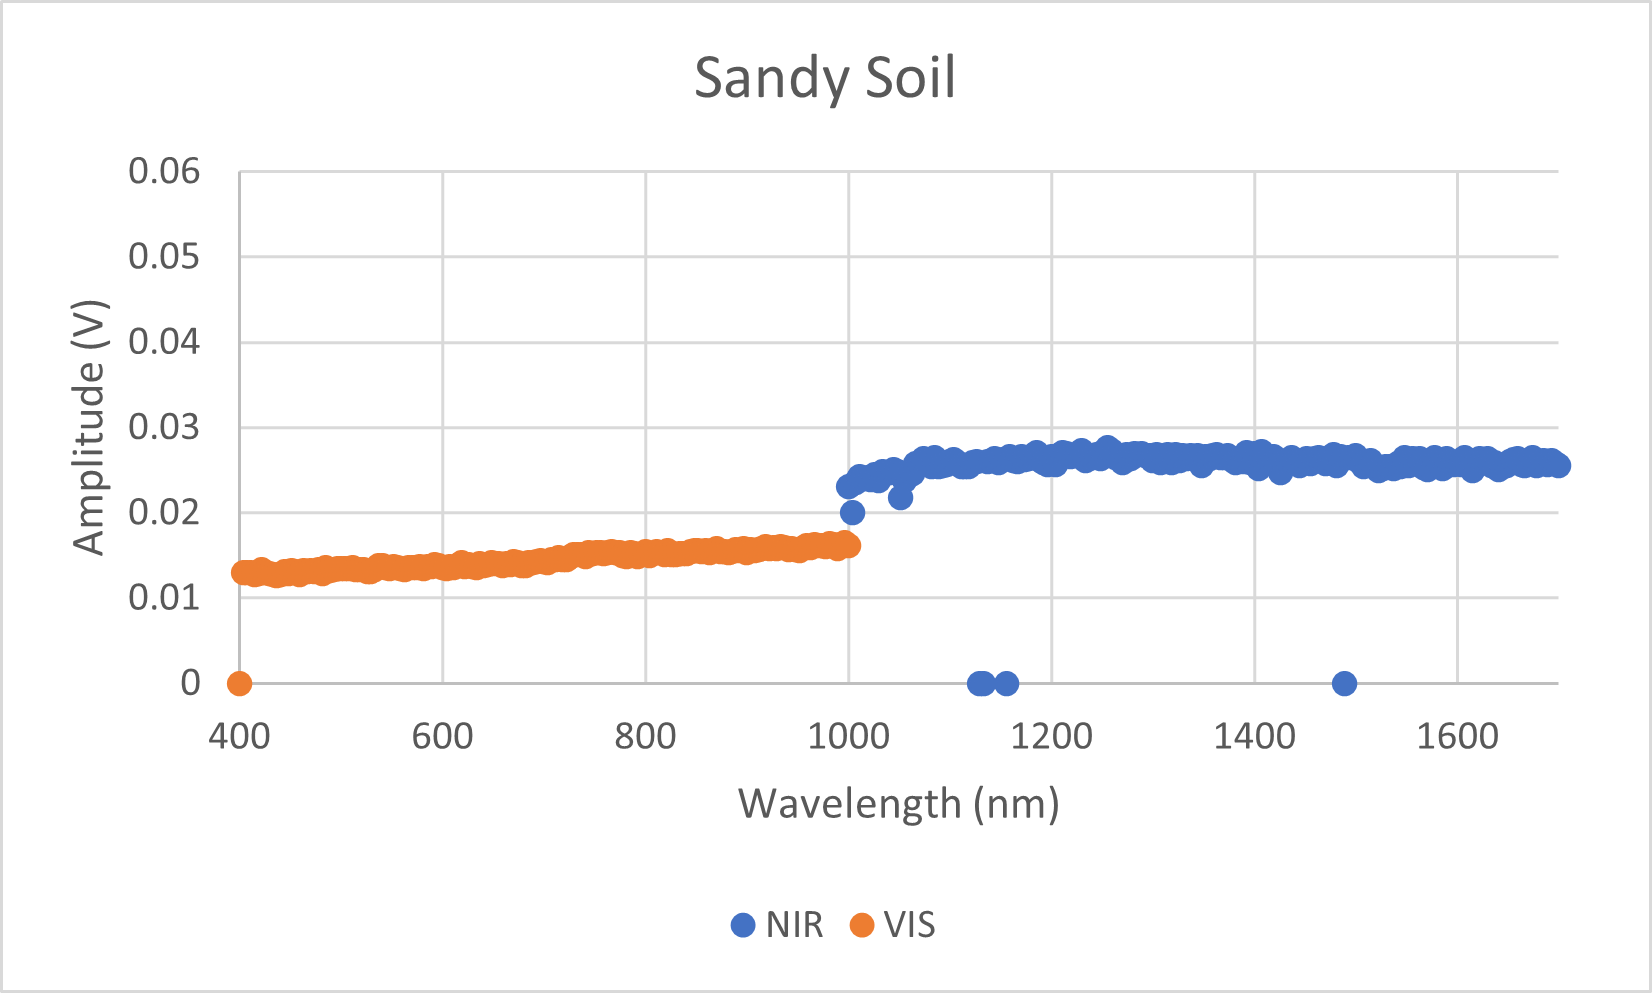
\includegraphics[width=\linewidth]{images/Data3.png}
   \caption{Spectrograph of a dry, unfertilized Sandy Soil}
\end{figure}
Each dataset has been truncated to clarify the region measured by each sensor, though otherwise there was much overlap. The wavelengths were assigned to captures by position, with the initial position of 400nm being measured from the initial position of the sensor circuitry, the rest of the values being extrapolated from there. As is clear from the spectrographs, there is a dramatic difference between the spectral content of the fertilized soil and the sandy soil. The spectral resolution of the system was set with a tape slit over the visible sensor, however this can be improved on greatly. Another area of limitation was the number of datapoints captured. While Web interfacing is still unimplemented, the memory on the microcontroller limits the size of each scan. With a tighter sensor slit and finer steps between captures, the spectrometer should achieve a spectral resolution of >5nm. This will allow for high precision scanning on many samples for calibration.
As of now, the major subsystems are all interfacing with each other to produce a genuine product, a spectrograph generating garden bed with infrastructure for automation and scaling.
\bibliographystyle{ieeetr}
\bibliography{references/sensing}
\end{document}